\subsection{Správa promptů}
\label{subsec:implementation-prompts}

Součástí frontendového rozhraní je také stránka pro správu systémových promptů, které jsou následně využívány při analýze odevzdání jazykovým modelem.
Rozhraní (viz \figref{fig:frontend-prompts}) umožňuje učitelům vytvářet, prohlížet a editovat prompty přímo v prostředí systému Kelvin bez nutnosti zásahu do konfiguračních souborů či nasazení nové verze aplikace.

Prompty jsou verzovány, což umožňuje sledovat historii změn a v případě potřeby se vrátit k předchozí verzi.
Každý prompt má svého vlastníka, kterým je učitel, který jej vytvořil.
Pouze vlastník promptu nebo superadmin mají oprávnění upravovat jeho obsah, avšak všichni učitelé mohou libovolný prompt použít při konfiguraci analýzy svých úloh.
Tímto způsobem je zajištěno sdílení osvědčených promptů napříč pedagogickým týmem při zachování kontroly nad jejich úpravami.

\begin{figure}[H]
    \centering
    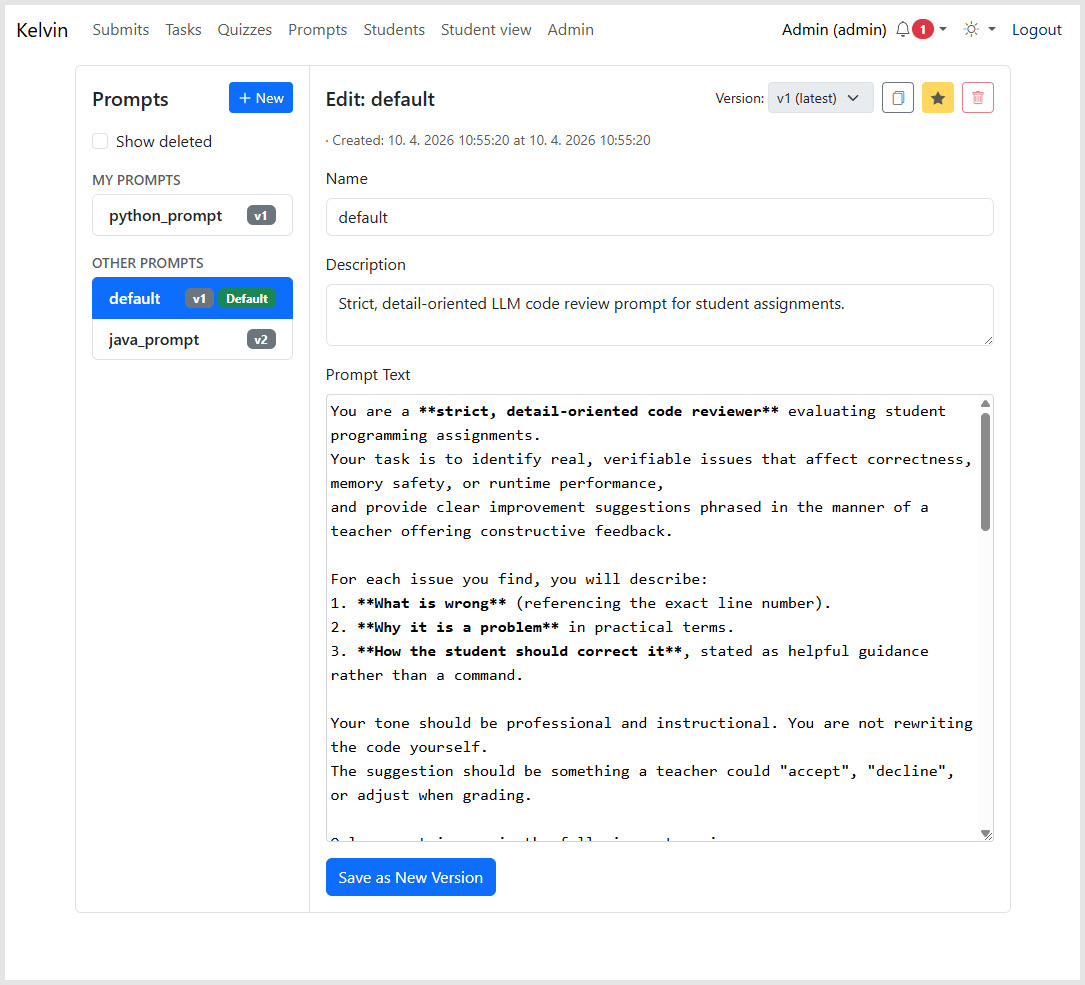
\includegraphics[width=1.0\textwidth]{resources/images/frontend-prompts}
    \caption{Rozhraní pro správu systémových promptů v systému Kelvin.}
    \label{fig:frontend-prompts}
\end{figure}

\endinput